\documentclass[a4paper,11pt]{article}

\usepackage[utf8]{inputenc} \usepackage[T1]{fontenc}
\usepackage{fancyhdr} \usepackage{graphicx,subfig} \usepackage{lastpage}
\usepackage{amssymb,amsmath} \usepackage{siunitx} \usepackage[nodayofweek]{datetime}
\usepackage[top=3.5cm,bottom=2.5cm,left=3cm,right=3cm,headheight=40pt]{geometry}
\usepackage{parskip} \usepackage{float} \usepackage{enumitem} \pagestyle{fancy}
\usepackage[colorlinks=true,allcolors=blue]{hyperref} \hypersetup{
	pdfauthor={Michaël Defferrard},
	pdftitle={Project stage 3: Interaction \& Animation},
	pdfsubject={Introduction to Computer Graphics}
}

\lhead{Introduction to Computer Graphics\\Project stage 3: Interaction \& Animation\\Group 19}
\chead{\hspace{2.5cm}EPFL\\\hspace{2.5cm}\shortdate\today\\\hspace{2.5cm}\thepage/\pageref{LastPage}}
\rhead{Michaël \textsc{Defferrard}\\Pierre \textsc{Fechting}\\Vu Hiep \textsc{Doan}}
\cfoot{}

\begin{document}


\section{Overview}

This report presents our advancement on the third part of the project : interaction and animation. During all the run of the project, we focused on code architecture and quality rather than quantity. It would have been impossible to implement every single idea we had about the project anyway.
%At this stage, we realized that we are better technicians than artists.

We did implement all the basic

\section{Implementation}

\subsection{Basics}

\subsection{Advanced}


\section{Improvements on last stage}

\subsection{Code cleanup}

As this hand-in is the last opportunity to modify our code, we put great effort in improving its quality by cleaning it up, including comments. A great job was done to functionalize shader code. As a side effect, we did also discover some little mistakes. We did also refactor most of the code to encompass our new object oriented architecture introduced in stage 2. In overall, code quality has greatly improved.

\subsection{Lightning}

Phong shading was improperly implemented at stage 2. The material texture was only used to compute the ambient color. The diffuse and specular colors were fixed for all the terrain. Probably a reminiscent of stage 1. This is now fixed. We first retrieve material color properties from textures. The retrieved color is then split across the three lightnings (ambient, diffuse and specular) with the help of coefficients which some up to 1. The specular lightning coefficient is non-zero for water only. The water uses two normals : a normalmap for diffuse lightning (this is used to create the impression of water movement) and a (0,0,1) normal for specular lightning (this is used to create the impression of sun light reflection).

The light direction was defined in stage 2 to be the same for all the vertices. This defines it as a directional light. It was changed to a spot light (or point light in the lightning context), to be coherent with shadowing. The shadowmap is indeed computed using perspective projection, not orthographic.

\subsection{Water animation}


\subsection{Vertices object}

To achieve better modulation, we have separated the vertices creation code into a class hierarchy. The \texttt{Vertices} base class is an abstract class, declaring only virtual methods, which defines the interface. The \texttt{VerticesQuad}, \texttt{VerticesGrid} and \texttt{VerticesSkybox} inherit from it and implement the \texttt{generate} \texttt{draw} and \texttt{clean} methods which are specific to them. This design allows more than one \text{RenderingContext} object to share a \texttt{Vertices} object. The \texttt{Terrain} and \texttt{Shadowmap} makes use of this. It also offers better source code modularity.

\subsection{Heightmap}

The heightmap texture was configured with the default heuristic for out-of-range values. This default is to wrap around the texture (\texttt{GL\_REPEAT}) which creates artifacts at the borders of the terrain (fig.~\ref{heightmap_artifacts}). Clamping the texture coordinates (\texttt{GL\_CLAMP\_TO\_EDGE}) to the [0,1] range eliminates the artifacts (fig.~\ref{heightmap_ok}).

\begin{figure}[ht]
	\centering
	\subfloat[With artifacts at the border]{
		\label{heightmap_artifacts}
		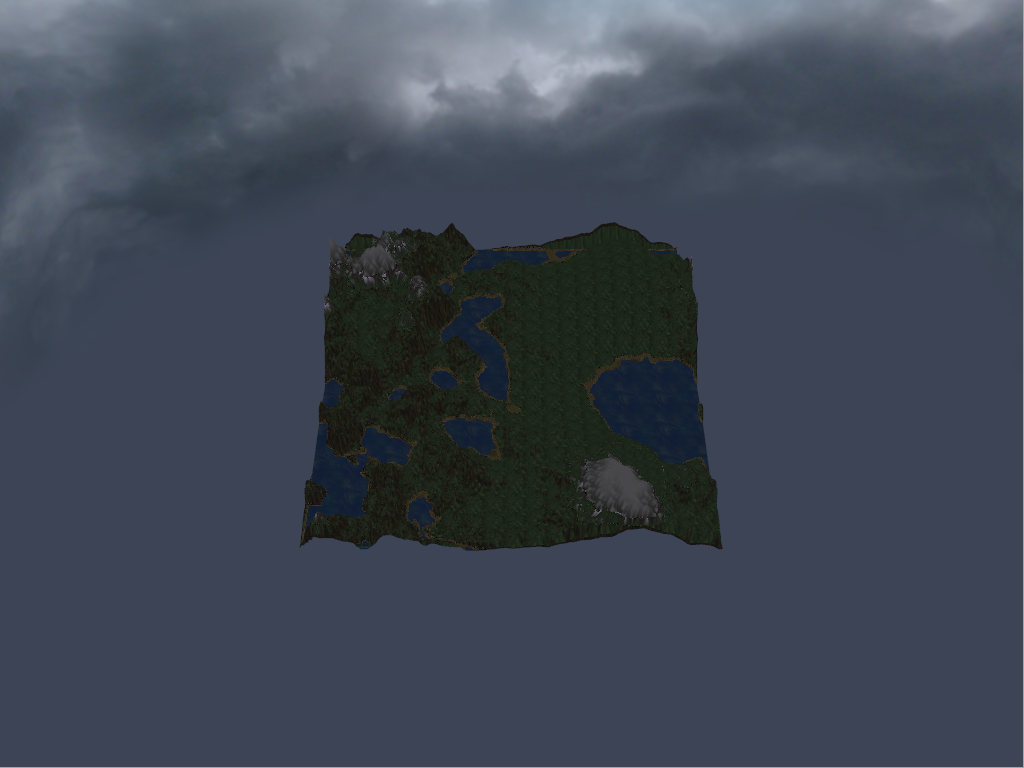
\includegraphics[height=4cm]{{{img_stage3/heightmap_artifacts}}}
	} \quad
	\subfloat[Without artifacts]{
		\label{heightmap_ok}
		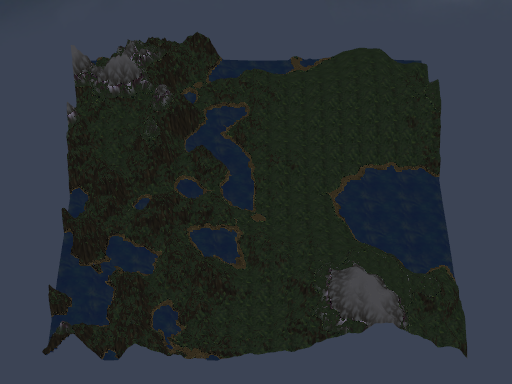
\includegraphics[height=4cm]{{{img_stage3/heightmap_ok}}}
	}
	\caption{Heightmap}
	\label{heightmap}
\end{figure}

The heightmap code was also refactored to accommodate our new object oriented architecture. This resulted in a cleaner design and better readability as well as some improvements of the generic code.

Another improvement of the heightmap code is that the \texttt{position} vector is now a \texttt{vec2} instead of a \texttt{vec3} as the vertex z position on a quad is 0 anyway. This saves some GPU memory bandwidth.

\section{Results}


\end{document}
